\documentclass[11pt,a4paper]{report}

% Aberstwyth dissertation LaTeX Template
% Authors: Dr. Hannah Dee (hmd1@aber.ac.uk), Neil Taylor (nst@aber.ac.uk)
% This has been adapted from the Leeds Thesis template and the 
% Group Project template for Computer Science in Aberystywth University.
% 
% All comments and suggestions welcome.
%
% Template designed to be used with pdflatex: it may need alteration to
% run with a different LaTeX engine

% To build document on the unix command line, run four commands:
 
% pdflatex dissertation
% bibtex dissertation
% pdflatex dissertation
% pdflatex dissertation

% you will end up with dissertation.pdf 
\usepackage{mmp}

% the following packages are used for citations - You only need to include one. 
%
% Use the cite package if you are using the numeric style (e.g. IEEEannot). 
% Use the natbib package if you are using the author-date style (e.g. authordate2annot). 
% Only use one of these and comment out the other one. 
%\usepackage{cite}
\usepackage{natbib}

% Use the following to selectively exclude chapters
%\includeonly{cover,abstract,acknowledge,declare,chapter1,chapter2}

\begin{document}

% all of the include directives below refer to tex files
% so 
\title{MapWars: Location-Aware Multi-Player Mobile Game}

% Your name
\author{Luke Ward}

% Your email 
\authoremail{luw9@aber.ac.uk}

\degreeschemecode{G400} %e.g. G400 
\degreeschemetitle{Computer Science} % e.g. Computer Science
\degreetype{BSc}

\modulecode{CS39440} % i.e. CS39440, CC39440, CS39620
\moduletitle{Major Project} % i.e. Major Project or Minor Project

\date{25th March 2013} % i.e. the date of this version of the report

\status{Draft} % Use draft until you create the release version. Then, change this to Release.
\version{1.0}

%The title and name of your supervisor.
\supervisor{Dr./Prof. My Supervisor} 

%The email for your supervisor. 
\supervisoremail{rzz@aber.ac.uk}

\maketitle



 includes cover.tex - to change the content,
% edit the tex file

\pagenumbering{roman}

% This is the front page

\title{MapWars: Location-Aware Multi-Player Mobile Game}

% Your name
\author{Luke Ward}

% Your email 
\authoremail{luw9@aber.ac.uk}

\degreeschemecode{G400} %e.g. G400 
\degreeschemetitle{Computer Science} % e.g. Computer Science
\degreetype{BSc}

\modulecode{CS39440} % i.e. CS39440, CC39440, CS39620
\moduletitle{Major Project} % i.e. Major Project or Minor Project

\date{25th March 2013} % i.e. the date of this version of the report

\status{Draft} % Use draft until you create the release version. Then, change this to Release.
\version{1.0}

%The title and name of your supervisor.
\supervisor{Dr./Prof. My Supervisor} 

%The email for your supervisor. 
\supervisoremail{rzz@aber.ac.uk}

\maketitle



                        

% Set up page numbering
\pagestyle{empty}

% declarations of originality 
\thispagestyle{empty}

%%%
%%% You must sign the declaration of originality. 
%%%
\begin{center}
    {\LARGE\bf Declaration of originality}
\end{center}

In signing below, I confirm that:

\begin{itemize}
\item{This submission is my own work, except where clearly
indicated.  }

\item{I understand that there are severe penalties for plagiarism 
and other unfair practice, which can lead to loss of marks
or even the withholding of a degree. }
 
\item{I have read the sections on unfair practice in the Students' 
Examinations Handbook and the relevant sections of the 
current Student Handbook of the Department of Computer 
Science.}
 
\item{I understand and agree to abide by the University's
regulations governing these issues.}
\end{itemize}

\vspace{3em}
Signature ............................................................  \\

\vspace{1em}
Date ............................................................ \\

%%% 
%%% We would like to make a selection of final reports available to students that take 
%%% this module in future years. To enable us to do this, we require your consent. You 
%%% are not required that you do this, but if you do give your consent, then we will have 
%%% the option to select yours as one of a number of reports as examples for other 
%%% students. If you would like to give your consent, then please include the following 
%%% text and sign below. If you do not wish to give your consent, please remove this 
%%% from your report. 
%%%
\vspace{5em}
\begin{center}
    {\LARGE\bf Consent to share this work}
\end{center}

In signing below, I hereby agree to this dissertation being made available to other
students and academic staff of the Aberystwyth Computer Science Department.  

\vspace{3em}
Signature ............................................................  \\

\vspace{1em}
Date ............................................................ \\

               

\thispagestyle{empty}

\begin{center}
    {\LARGE\bf Acknowledgements}
\end{center}

I am grateful to...

I'd like to thank...
 % Acknowledgements
\thispagestyle{empty}

\begin{center}
    {\LARGE\bf Abstract}
\end{center}

MapWars is the culmination of an investigation into the feasibility of creating a location-aware, multi-player \gls{rts} game for a mobile platform. Consideration about which platform to support is presented with the final decision being to focus on Google's Android operating system.

The game combines strategic game play against multiple players in a persistent environment, where game play is based on map of Earth and users are restricted in game to their real world location. Giving each user the capability to create their own army and battle against other players within their local area.

At the same time consideration was made to protect each users privacy and create a fair gaming experience. Thus different techniques on how to prevent crafted requests designed to circumnavigate limits placed in the Android client.

                 % Abstract

\pagenumbering{roman}
\pagestyle{fancy}
\fancyhead{}
\fancyfoot[C]{\thepage}
\renewcommand{\headrulewidth}{0 pt}
\renewcommand{\chaptermark}[1]{\markboth{#1}{}}

\tableofcontents   
\newpage
\listoffigures
\newpage 
\listoftables
\newpage

% Set up page numbering
\pagenumbering{arabic}

\setchapterheaderfooter

% include the chapters
\chapter{Background \& Objectives}

This section should pick-up material from your progress report and enhance it based on the feedback and also your additional experience up to now. 

\textbf{Note: All of the sections and text in this example are for illustration purposes. The main Chapters are a good starting point, but the content and actual sections that you include are likely to be different.}
%\addcontentsline{toc}{chapter}{Development Process}
\chapter{Development Process}

You need to describe briefly the life cycle model that you used. Do not force your project into the waterfall model if it is better described by prototyping or some other evolutionary model. You do not need to write about all of the different process models that you are aware of. Focus on the process model that you have used. It is possible that you needed to adapt an existing process model to suit your project; clearly identify what you used and how you adapted it for your needs.

In most cases, the agreed objectives or requirements will be the result of a compromise between what would ideally have been produced and what was felt to be possible in the time available. A discussion of the process of arriving at the final list is usually appropriate.

You should briefly describe the design method you used and any support tools that you used. You should discuss your choice of implementation tools - programming language, compilers, database management system, program development environment, etc.

\section{Introduction}
Introduce the specific model that you chose to use. 

\section{Modifications}
Did you have to modify the model to suit a one-person project. If so, what did you change and why? 

\chapter{Design}



You should concentrate on the more important aspects of the design. It is essential that an overview is presented before going into detail. As well as describing the design adopted it must also explain what other designs were considered and why they were rejected.

The design should describe what you expected to do, and might also explain areas that you had to revise after some investigation.

Typically, for an object-oriented design, the discussion will focus on the choice of objects and classes and the allocation of methods to classes. The use made of reusable components should be described and their source referenced. Particularly important decisions concerning data structures usually affect the architecture of a system and so should be described here.

How much material you include on detailed design and implementation will depend very much on the nature of the project. It should not be padded out. Think about the significant aspects of your system. For example, describe the design of the user interface if it is a critical aspect of your system, or provide detail about methods and data structures that are not trivial. Do not spend time on long lists of trivial items and repetitive descriptions. If in doubt about what is appropriate, speak to your supervisor.


\section{Overall Architecture}

\section{Some detailed design}

\subsection{Even more detail}

\section{User Interface}

\section{Other relevant sections}
\chapter{Implementation}

The implementation should look at any issues you encountered as you tried to implement your design. During the work, you might have found that elements of your design were unnecessary or overly complex, perhaps third party libraries were available that simplified some of the functions that you intended to implement. If things were easier in some areas, then how did you adapt your project to take account of your findings?

It is more likely that things were more complex than you first thought. In particular, were there any problems or difficulties that you found during implementation that you had to address? Did such problems simply delay you or were they more significant? Your implementation might well be described in the same chapter as Problems (see below).


\chapter{Testing}

Detailed descriptions of every test case are definitely not what is required here. What is important is to show that you adopted a sensible strategy that was, in principle, capable of testing the system adequately even if you did not have the time to test the system fully.

Have you tested your system on 'real users'? For example, if your system is supposed to solve a problem for a business, then it would be appropriate to present your approach to involve the users in the testing process and to record the results that you obtained. Depending on the level of detail, it is likely that you would put any detailed results in an appendix.

\section{Overall Approach to Testing}

\section{Automated Testing}

\subsection{Unit Tests}

\subsection{User Interface Testing}

\subsection{Stress Testing}

\subsection{Other types of testing}

\section{Integration Testing}

\section{User Testing}
\chapter{Evaluation}

Examiners expect to find in your dissertation a section addressing such questions as:

\begin{itemize}
   \item Were the requirements correctly identified? 
   \item Were the design decisions correct?
   \item Could a more suitable set of tools have been chosen?
   \item How well did the software meet the needs of those who were expecting to use it?
   \item How well were any other project aims achieved?
   \item If you were starting again, what would you do differently?
\end{itemize}

Such material is regarded as an important part of the dissertation; it should demonstrate that you are capable not only of carrying out a piece of work but also of thinking critically about how you did it and how you might have done it better. This is seen as an important part of an honours degree. 

There will be good things and room for improvement with any project. As you write this section, identify and discuss the parts of the work that went well and also consider ways in which the work could be improved. 

The critical evaluation can sometimes be the weakest aspect of most project dissertations. We will discuss this in a future lecture and there are some additional points raised on the project website. 
% add any additional chapters here

\setemptyheader
\addcontentsline{toc}{chapter}{Appendices}
\chapter*{Appendices}
\pagebreak

% start the appendix - sets up different numbering
\fancypagestyle{plain}{%
%\fancyhf{} % clear all header and footer fields
\fancyhead[L]{\textsl{Appendix\ \thechapter}}
\fancyhead[R]{\textsl{\leftmark}}}

\appendix
\fancyhead[L]{\textsl{Appendix\ \thechapter}}
\fancyhead[R]{\textsl{\leftmark}}
\fancyhead[C]{}
\fancyfoot[C]{\thepage}
\renewcommand{\headrulewidth}{0.4pt}
\renewcommand{\chaptermark}[1]{\markboth{#1}{}}

\fancyhead[L]{\textsl{Appendix\ \thechapter}}
\fancyhead[R]{\textsl{\leftmark}}
\fancyfoot[C]{{\thepage} of \pageref{LastPage}}

% include any appendices here
\chapter{Third-Party Code and Libraries}

If you have made use of any third party code or software libraries, i.e. any code that you have not designed and written yourself, then you must include this appendix. 

As has been said in lectures, it is acceptable and likely that you will make use of third-party code and software libraries. The key requirement is that we understand what is your original work and what work is based on that of other people. 

Therefore, you need to clearly state what you have used and where the original material can be found. Also, if you have made any changes to the original versions, you must explain what you have changed. 


\chapter{Class diagram}\label{ap_class}

\begin{figure}[H]
  \centering
  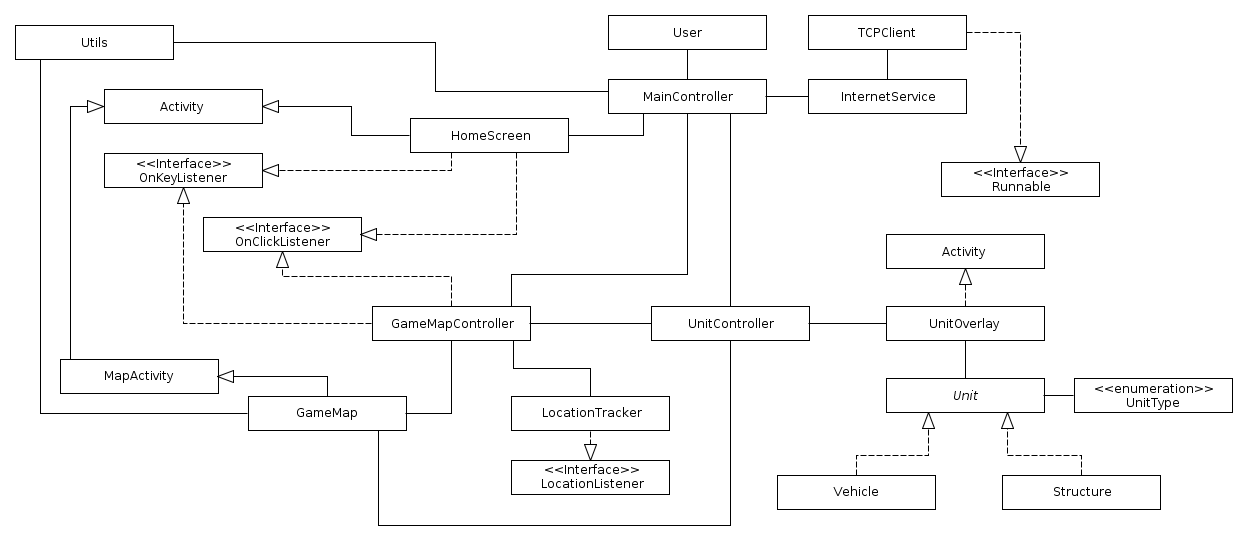
\includegraphics[height=0.3\textheight, angle=90]{Images/diagrams/class.png}
\end{figure}



\chapter{Server Testing Data Generator}\label{server_testing}

\begin{verbatim}
#!/usr/bin/env python
import socket
import sys
import time
import re
import json


HOST = 'localhost'
PORT = 4565

sess = None
userID = None

try:
  sock = socket.socket(socket.AF_INET, socket.SOCK_STREAM)
  sock.connect((HOST, PORT))
except socket.error, msg:
  sys.stderr.write("[ERROR] %s\n" % msg[1])
  sys.exit(1)


while True:
  n = raw_input("> ")

  msgDic = dict()

  if n == "exit":
    break  # stops the loop
  else:
    match = re.findall("[^\s]+", n, re.M|re.I)
    if match:
      if match[0] == 'login':
        msgDic['action'] = "user.login"
        msgDic['user'] = match[1]
        msgDic['pass'] = match[2]
      elif match[0] == 'register':
        msgDic['action'] = "user.register"
        msgDic['user'] = match[1]
        msgDic['pass'] = match[2]
        msgDic['email'] = match[3]
      elif match[0] == 'location':
        msgDic['action'] = "user.location"

        if len(match) == 3:
          msgDic['lat'] = match[1]
          msgDic['lon'] = match[2]
        else:
          msgDic['lat'] = '52.35184333541474'
          msgDic['lon'] = '-1.966477632522583'
      elif match[0] == 'unit':
        msgDic['action'] = "unit.create"
        msgDic['type'] = match[1]
        msgDic['lat'] = match[2]
        msgDic['lon'] = match[3]
      elif match[0] == 'move':
        msgDic['action'] = "unit.move"
        msgDic['id'] = match[1]
        msgDic['lat'] = match[2]
        msgDic['lon'] = match[3]
      else:
        continue
      
      if sess:
        msgDic['sess'] = sess
      if userID:
        msgDic['userID'] = userID

      msg = json.dumps(msgDic)
      print '\x1b[38;5;15m' + "S " + msg + '\033[0m'
      sock.send(msg)


    else:
      continue


  rec = sock.recv(2048)
  try:
    data = json.loads(rec)

    #check for session data
    if data['action'] == 'user.login' and data['status'] == 1:
      sess = data['sess']
      #sess = 'cat'
      userID = data['userID']

    if data['status'] == 1:
      print '\x1b[38;5;46m' + "R " + rec + '\033[0m'
    else:
      print '\x1b[38;5;160m' + "R " + rec + '\033[0m'
  except ValueError:
    print rec


sock.close()

sys.exit(0)

\end{verbatim}
\chapter{Class diagram}\label{ap_class}

\begin{figure}[H]
  \centering
  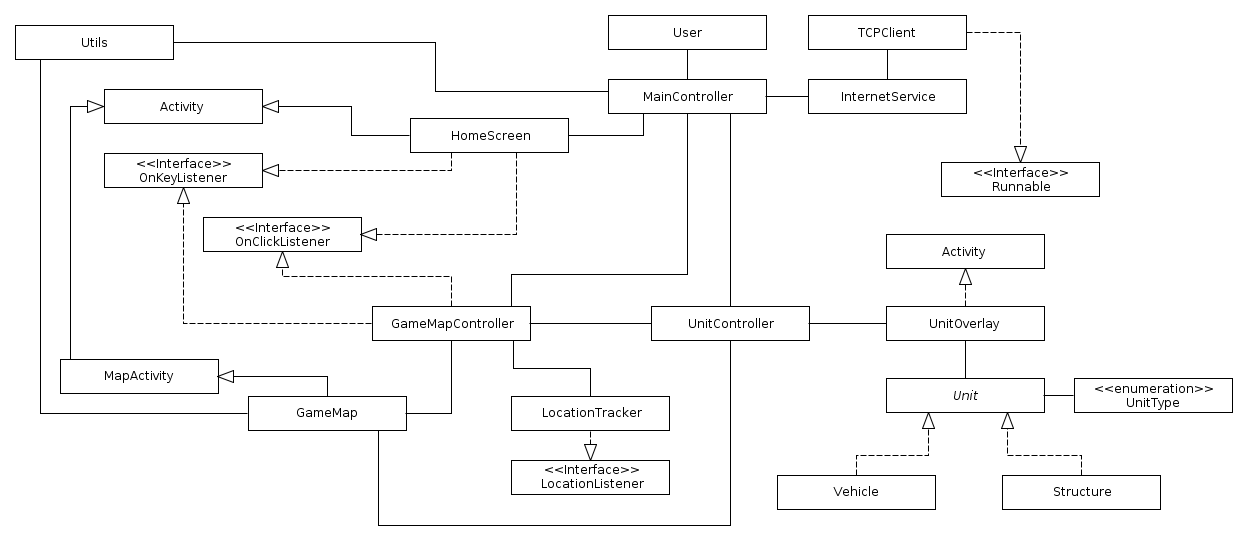
\includegraphics[height=0.3\textheight, angle=90]{Images/diagrams/class.png}
\end{figure}



\chapter{Server Testing Data Generator}\label{ap_class}

\begin{verbatim}
#!/usr/bin/env python
import socket
import sys
import time
import re
import json


HOST = 'localhost'
PORT = 4565

sess = None
userID = None

try:
  sock = socket.socket(socket.AF_INET, socket.SOCK_STREAM)
  sock.connect((HOST, PORT))
except socket.error, msg:
  sys.stderr.write("[ERROR] %s\n" % msg[1])
  sys.exit(1)


while True:
  n = raw_input("> ")

  msgDic = dict()

  if n == "exit":
    break  # stops the loop
  else:
    match = re.findall("[^\s]+", n, re.M|re.I)
    if match:
      if match[0] == 'login':
        msgDic['action'] = "user.login"
        msgDic['user'] = match[1]
        msgDic['pass'] = match[2]
      elif match[0] == 'register':
        msgDic['action'] = "user.register"
        msgDic['user'] = match[1]
        msgDic['pass'] = match[2]
        msgDic['email'] = match[3]
      elif match[0] == 'location':
        msgDic['action'] = "user.location"

        if len(match) == 3:
          msgDic['lat'] = match[1]
          msgDic['lon'] = match[2]
        else:
          msgDic['lat'] = '52.35184333541474'
          msgDic['lon'] = '-1.966477632522583'
      elif match[0] == 'unit':
        msgDic['action'] = "unit.create"
        msgDic['type'] = match[1]
        msgDic['lat'] = match[2]
        msgDic['lon'] = match[3]
      elif match[0] == 'move':
        msgDic['action'] = "unit.move"
        msgDic['id'] = match[1]
        msgDic['lat'] = match[2]
        msgDic['lon'] = match[3]
      else:
        continue
      
      if sess:
        msgDic['sess'] = sess
      if userID:
        msgDic['userID'] = userID

      msg = json.dumps(msgDic)
      print '\x1b[38;5;15m' + "S " + msg + '\033[0m'
      sock.send(msg)


    else:
      continue


  rec = sock.recv(2048)
  try:
    data = json.loads(rec)

    #check for session data
    if data['action'] == 'user.login' and data['status'] == 1:
      sess = data['sess']
      #sess = 'cat'
      userID = data['userID']

    if data['status'] == 1:
      print '\x1b[38;5;46m' + "R " + rec + '\033[0m'
    else:
      print '\x1b[38;5;160m' + "R " + rec + '\033[0m'
  except ValueError:
    print rec


sock.close()

sys.exit(0)

\end{verbatim}

\fancypagestyle{plain}{%
   \fancyhead{} %[C]{Annotated Bibliography}
   \fancyfoot[C]{{\thepage} of \pageref{LastPage}} % except the center
   \renewcommand{\headrulewidth}{0pt}
   \renewcommand{\footrulewidth}{0pt}
}

\setemptyheader

\nocite{*} % include everything from the bibliography, irrespective of whether it has been referenced.

% the following line is included so that the bibliography is also shown in the table of contents. There is the possibility that this is added to the previous page for the bibliography. To address this, a newline is added so that it appears on the first page for the bibliography. 
\addcontentsline{toc}{chapter}{Annotated Bibliography} % Adds References to contents page

%
% example of including an annotated bibliography. The current style is an author date one. If you want to change, comment out the line and uncomment the subsequent line. You should also modify the packages included at the top (see the notes earlier in the file) and then trash your aux files and re-run. 
\bibliographystyle{authordate2annot}
%\bibliographystyle{IEEEannot}
\renewcommand{\bibname}{Annotated Bibliography} 
\bibliography{References/references} % References file


\end{document}
